\documentclass[sigconf,review,anonymous]{acmart}

\usepackage{tikz}
\usetikzlibrary{arrows.meta,positioning}

\acmConference[CGO 2027]{International Symposium on Code Generation and
Optimization}{March 20--24, 2027}{Salt Lake City, UT, USA}
\acmDOI{}
\acmISBN{}
\settopmatter{printacmref=false}
\renewcommand\footnotetextcopyrightpermission[1]{}
\pagestyle{plain}

\begin{document}

\title{Measured, Not Assumed: Four Ways an Optimizer's Own Evidence Misleads It}

\author{Anonymous Author(s)}
\affiliation{\institution{Anonymous Institution}\country{}}

\begin{abstract}
We report four independent findings from building and evaluating a
correctness-gated loop-vectorizing optimizer that targets dependence
structure a compiler cannot prove safe to reorder. None of them is a speedup:
the optimizer's own analysis ceiling (52.3\%) sits below the published TSVC2
vectorization record (56.0\%, on incomparable hardware), and pointed at ten
repositories it did not author, its transformation catalogue matched zero
loops out of 10{,}777. Instead, each finding is a case where the optimizer's
own evaluation apparatus -- the cost model that priced its capabilities, the
benchmark it was tuned against, the timing rig that judged a transformation,
the tool that checked its own correctness claim -- was the wrong witness to
trust, and something external to the producing code path was required to
catch it. (1) A capability-pricing model computed at the granularity of a
declared \emph{genus} priced a missing feature at +599 loops on a held-out
corpus; the \emph{species} actually built to fill that gap delivered +14, a
43$\times$ overstatement recorded prospectively, before the build, not
rationalized after it. (2) Running the same pipeline against code it did not
author surfaced five wrong-code classes hiding behind a coincidence uniform
across its entire home benchmark, plus three more found while extending the
tool and by an independent checker. (3) A performance gate that reused
degenerate state across repetitions did not merely misestimate a
transformation's speedup -- it inverted the decision, publishing a
regression as a 1.56$\times$ accept. (4) An independent witness/validator
layer, sharing no code with the component it checks, found a correctness bug
on its first run that the producing harness structurally could not see. We
argue these are not incidental engineering bugs but a pattern: self-measured
evidence about an optimizer's own value systematically overstates it, and
each fix required consulting something the producing system did not build.
\end{abstract}

\maketitle

\section{Introduction}

This is not a speedup paper. We say so first because it is the question a
reader will otherwise spend the rest of the paper waiting to have answered.
The loop-vectorizing optimizer this paper reports on does not beat a tuned
baseline: its best derived ceiling on TSVC2 (52.3\%) is below the published
record for the suite (56.0\%, on different, wider-vector hardware, and so not
even a comparable number); and pointed at ten real repositories it never saw
during development, its transformation catalogue -- distribution, dead-store
elimination, preloading, peeling, predicated execution -- matched exactly
zero of 10{,}777 loops. If this paper's contribution were a performance
result, it would end here.

Its contribution is four findings about how the optimizer's own evaluation
apparatus misled its builders, and how each was caught. All four share a
structure: some component of the system -- a cost model, a benchmark, a
timing rig, a correctness checker -- was consulted to answer a question
about the system's own value, and in each case something \emph{external} to
that component was needed before the answer could be trusted.

\begin{itemize}
\item \textbf{C1.} A capability-pricing instrument priced a declared
refusal at the level of a \emph{genus} -- a broad, named class of code the
optimizer cannot yet handle -- and that price did not forecast what building
one \emph{species} of that genus would deliver. The overstatement was
43$\times$ (\S\ref{sec:c1}), and it was measured \emph{prospectively}: the
price was recorded before the species was built, not fit to the outcome
afterward.
\item \textbf{C2.} Running the pipeline against ten repositories it was
never tuned on surfaced eight wrong-code classes across its correctness
machinery, five of them hiding behind a coincidence true of every loop in
its own benchmark simultaneously -- and therefore invisible from inside that
benchmark by construction (\S\ref{sec:c2}).
\item \textbf{C3.} A performance gate whose timing loop reused state left
over from the previous repetition did not just produce a noisier number --
it inverted an accept/reject decision. A fixture published as a
1.56$\times$ speedup was, under a measurement that reset its input properly,
a 5.9$\times$ regression (\S\ref{sec:c3}).
\item \textbf{C4.} An independent witness-and-validator layer, built to
share no code with the component whose claims it checks, found a
correctness bug -- wrong output at a trip count the producing harness never
exercised -- on its first run (\S\ref{sec:c4}).
\end{itemize}

\begin{table*}[t]
\caption{The four findings, at a glance. Every number is machine-checked by
a single reproducible entry point, \texttt{just test}.}
\label{tab:summary}
\small
\begin{tabular}{@{}p{0.03\linewidth}p{0.40\linewidth}p{0.32\linewidth}p{0.15\linewidth}@{}}
\toprule
\textbf{\#} & \textbf{What was trusted, and shouldn't have been} & \textbf{What caught it} & \textbf{Magnitude} \\
\midrule
C1 & A genus-level capability price, read as a species-level forecast & A prospective build-then-compare, recorded before the fact & 599 vs.\ 14 (43$\times$) \\
\addlinespace
C2 & A benchmark's own internal uniformities, mistaken for coverage & Running unmodified on 10 unrelated repositories & 8 defect classes, 0/10{,}777 wins \\
\addlinespace
C3 & A timing rig that reused corrupted state across trials & Resetting input outside the timed region & 1.56$\times$ ACCEPT $\rightarrow$ 5.9$\times$ regression \\
\addlinespace
C4 & A correctness harness's own claim about its own output & A validator sharing no code with the producer & $-86 \rightarrow{}+50$ score, 1st run \\
\bottomrule
\end{tabular}
\end{table*}

We position these as a single argument rather than four anecdotes:
\emph{self-measurement is not evidence about a system, no matter how
carefully the self-measuring component is built.} A price, a benchmark rate,
a timing number, and a correctness claim are all, in this project's own
experience, systematically overstated when the thing producing the number is
also the thing being judged -- and in every one of the four cases, the fix
was not a better internal metric but an external check with no shared code
path to the thing it evaluates. \S\ref{sec:discussion} draws this out as a
set of prescriptions we believe generalize past this one optimizer.

The artifact backing all four findings is a single command
(\texttt{just test}) that reproduces every gate, witness, and pin referenced
in this paper end to end; we submit it as an available, though not yet
AE-badged, companion to this text.

\section{Background and Related Work}
\label{sec:background}

\paragraph{Loop vectorization and TSVC2.}
TSVC2~\cite{tsvc2} is the direct descendant of the Callahan--Dongarra--Levine
1988 test suite, one dependence pattern per named kernel. A 2025 study
directly relevant to our hardware target measured GCC, Clang, and ARM's own
compiler on both x86 and ARM, on the exact TSVC2 corpus we use, and reports
GCC 14.1.1 at 56.0\% (85/151) on A64FX/SVE-512~\cite{tsvc2-arm-x86}; we cite
this as the closest available apples-to-apples baseline throughout, and
disclose every time we do so that our own hardware (Apple M4, 128-bit NEON,
no general-purpose SVE) is not comparable to A64FX's 512-bit SVE lanes. No
external leaderboard exists for CPU-side, ARM-targeting loop vectorization:
the one venue that ever structurally matched this shape,
CompilerGym's~\cite{compilergym} LLVM instruction-count leaderboard, is
archived, and had taken no new submission for four years before its
archival. Every comparable system we are aware of -- Souper, STOKE,
Minotaur, Diospyros, Ansor -- self-reports on a self-chosen, published
corpus against named baseline compilers; that is the field's actual norm,
not a weaker position, and it is the norm this paper follows.

\paragraph{Correctness methodology.}
Diospyros~\cite{diospyros} synthesizes vectorized realizations for
fixed-size DSP kernels and validates them by \emph{translation
validation}: lowering both the scalar specification and the synthesized
vector code into a common imperative vector DSL and checking semantic
equivalence directly, rather than trusting a compiler's own claim. Our
correctness gate (a differential harness comparing an optimized realization
against an unoptimized reference across many input regimes) and our witness
layer (\S\ref{sec:c4}) are in the same spirit -- check the transformation's
actual behavior, not the tool's report of what it did -- though our witness
design borrows its scoring discipline directly from software verification
rather than from translation validation.

\paragraph{Evaluation methodology this paper extends.}
Two prior critiques of how program-optimization tools are evaluated
directly motivate C2--C4. Kalibera and Jones~\cite{kalibera-jones} argue
that a fixed noise margin, chosen from within-session variance, understates
real-world measurement noise by an order of magnitude or more; our own
machine-contention finding (\S\ref{sec:c3}) independently reproduces this on
a modern ARM laptop SoC rather than a server benchmark rig. Regehr et
al.~\cite{creduce} name ``the test-case validity problem'' for compiler
fuzzing -- that a supposedly-failing test case is often invalid for reasons
unrelated to the bug being chased -- fourteen years before an unrelated
project (ours) independently rediscovered three instances of the same
failure mode in its own measurement harness. SV-COMP's central discipline,
that a verification tool emits a \emph{witness} and a separately-built
\emph{validator} decides whether to believe it~\cite{svcomp-witnesses}, is
the direct design source for C4. Neural-architecture-search's own
performance-estimation literature -- zero-cost, training-free proxies that
price a candidate from its declared structure rather than by building
it~\cite{nas-survey} -- is the closest existing frame for what C1's pricing
instrument is: our finding is that the granularity such a proxy is priced
at, not merely its accuracy, is itself a source of systematic error. We
position C1 and C3 as two further instances of this same lineage --
optimizer evaluation infrastructure that looked correct until checked
externally -- rather than as a claim that either is entirely novel in kind.

We do not survey learned/ML-guided compilation optimization (MLGO, Ansor,
TenSet) in depth: these target a different decision surface (inlining and
register allocation, or DNN tensor-program scheduling) evaluated on
different hardware, and a prior survey we conducted found no shared metric
or corpus that would make a numeric comparison meaningful rather than
misleading~\cite{mlgo,ansor,tenset}.

\section{System and Experimental Setup}
\label{sec:setup}

The optimizer under study is a correctness-gated pipeline: lift a C loop's
dependence structure from source using libclang, classify it, choose a
transformation from a small catalogue (loop distribution over an
Allen--Kennedy strongly-connected-component decomposition, dead-store
elimination, preloading, peeling with scalar expansion, and predicated
execution for guarded assignments), verify the result correct against a
differential harness run over many input regimes, verify it faster against a
timing gate, and accept or reject. All measurements in this paper were taken
on an Apple M4 (4 performance + 6 efficiency cores, 128-bit NEON, no
general-purpose SVE).

\begin{figure*}[t]
\centering
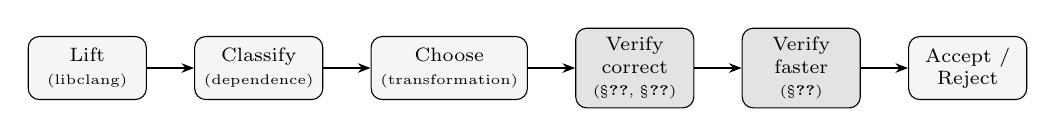
\begin{tikzpicture}[
  node distance=6mm,
  box/.style={draw, rounded corners, align=center, minimum height=8mm,
    minimum width=15mm, font=\scriptsize, fill=gray!8},
  gate/.style={box, fill=gray!22},
  arr/.style={-{Stealth[length=1.6mm]}, thick}
]
\node[box] (lift) {Lift\\\tiny(libclang)};
\node[box, right=of lift] (classify) {Classify\\\tiny(dependence)};
\node[box, right=of classify] (choose) {Choose\\\tiny(transformation)};
\node[gate, right=of choose] (correct) {Verify\\correct\\\tiny(\S\ref{sec:c2}, \S\ref{sec:c4})};
\node[gate, right=of correct] (fast) {Verify\\faster\\\tiny(\S\ref{sec:c3})};
\node[box, right=of fast] (accept) {Accept /\\Reject};
\draw[arr] (lift) -- (classify);
\draw[arr] (classify) -- (choose);
\draw[arr] (choose) -- (correct);
\draw[arr] (correct) -- (fast);
\draw[arr] (fast) -- (accept);
\end{tikzpicture}
\caption{The pipeline under study. Shaded stages are gates a candidate must
pass; the two we found broken (\S\ref{sec:c2}--\S\ref{sec:c4}) are the ones
this paper is actually about, not the transformation catalogue itself.}
\label{fig:pipeline}
\end{figure*}

\paragraph{TSVC2 headline.} Clang \texttt{-O3 -mcpu=native} alone vectorizes
64/151 = 42.4\% of TSVC2's kernels. Adding the pipeline recovers 10 further
kernels at measured speedups of 1.3--4.5$\times$ (quiet-machine
measurement, \S\ref{sec:c3}), for 74/151 = 49.0\%. The pipeline's own
derived analysis ceiling -- computed from its declared capabilities, not
asserted -- is 52.3\%, below the 56.0\% record on incomparable hardware
(\S\ref{sec:background}). We state this once, plainly, and do not revisit it
as a result: it is context for what follows, not a claim in its own right.

\paragraph{The repository-scale probe.} The same pipeline, unmodified, was
pointed at ten repositories it did not author and was never tuned against:
Opus, Vorbis, SpeexDSP, libsamplerate, Darknet, Genann, PolyBench/C, the NAS
Parallel Benchmarks, MILC (lattice QCD), and GSL -- 10{,}777 distinct loops
in total. \emph{Zero} were transformed. Reach and yield are independent
here: PolyBench, the canonical affine-loop benchmark, lifts (is even
analyzable by the dependence classifier) at only 7\%, the worst of the ten,
because its loops are multi-dimensional; GSL lifts at 91\%, the best, and
still yields no applicable transformation. This probe is not itself one of
the paper's four claims -- it is the instrument C1 and C2 were measured
with, and we describe it once here rather than re-deriving it in each
section that draws on it.

\section{C1: Genus-Level Prices Do Not Forecast Species-Level Delivery}
\label{sec:c1}

The pipeline declares its own reach as a vocabulary of named
\emph{capabilities} -- refused code shapes such as \texttt{body.control\_flow}
(a guarded assignment inside a loop body) or \texttt{access.multi\_dimensional}
-- each with an \texttt{admits}/\texttt{refuses} contract. Given this
vocabulary, a pricing tool derives, \emph{before any transformation is
built}, how many additional loops a chooser could recover if a given
capability were admitted: a zero-cost structural proxy in the spirit of
training-free neural-architecture-search performance
estimators~\cite{nas-survey}, priced from declared structure rather than
measured by execution.

Priced against the project's own in-repository TSVC2 corpus,
\texttt{body.control\_flow} ranked as a modest refusal. Re-derived on the
held-out corpus from the repository-scale probe (\S\ref{sec:setup}, 5{,}147
loops across the ten external repositories, none seen during tuning),
\texttt{body.control\_flow} was the \emph{top-ranked} refusal: +599 loops,
blocking 2{,}108 loops in total when compounded with other capabilities.
This was recorded as a prospective prediction, on disk, before any code
addressing the refusal was written -- the ordering that makes the number a
test of the pricing instrument rather than a post-hoc rationalization of
whatever happened to get built.

What was actually built, predicated execution, does not admit
\texttt{body.control\_flow} as a whole. It normalizes one \emph{species} of
it -- guarded assignments of the shape \texttt{if (P) lhs = rhs;} -- into a
select form, and refuses every other shape the genus contains: nested
guards, guarded non-assignment statements, early exits, unsafe speculation
under the guard. Measured on the identical held-out corpus the price was
computed against, this species delivered \textbf{+14} loops.

\[
\frac{599 \text{ priced}}{14 \text{ delivered}} \approx 43\times
\]

The arithmetic that produced 599 was not wrong -- it is the correct answer
to ``how many loops does \texttt{body.control\_flow}, as a whole, block.''
It is simply the wrong question to have asked before deciding what to build,
because most of the priced value was never reachable by any single species.
The single largest capability by price in the same held-out ranking,
\texttt{body.nested\_loop} at +2{,}888 loops, is not a species of
\texttt{body.control\_flow} at all -- it is a structurally unrelated
capability that happened to co-occur with control flow across the probe
corpus often enough to inflate the compounded estimate, a supermodularity
effect the pricing tool measured (+1{,}209 loops summed across capabilities
individually, versus +3{,}074 loops when priced jointly) but which the
genus-level framing obscures rather than explains.

The generalizable claim we draw is narrow and falsifiable: \emph{a
capability price computed at genus granularity should not be read as a
forecast of what building any one species of that genus will deliver,
because a heterogeneous genus's price is dominated by species that may never
be built.} Any optimizer that reports ``this refusal is worth $N$ recovered
cases'' should disclose the granularity $N$ was priced at relative to the
granularity of whatever gets built to address it.

\section{C2: Leaving the Benchmark Finds What the Benchmark Cannot}
\label{sec:c2}

The repository-scale probe (\S\ref{sec:setup}) found zero applicable
transformations, but it found something else: eight distinct wrong-code
classes in the pipeline's own machinery, none of which the project's home
benchmark (TSVC2, its ten probe loops, and its differential test suite) had
ever surfaced. We split them by how they were found, because the split
matters to the argument: only one set demonstrates that a home benchmark is
\emph{structurally} incapable of finding a given defect, and it is worth
distinguishing that set from ordinary bugs any further testing might have
caught eventually.

\paragraph{Five defects hiding behind a shared coincidence.} TSVC2's probe
loops -- the specific subset the correctness and dependence-classification
machinery was validated against during development -- are, as a set,
uniform along five independent axes simultaneously: every loop steps by 1;
every loop ascends; every dead store is written last in its iteration; every
array is named by a plain identifier rather than a struct member or pointer
expression; and every loop stays inside the differential harness's own
allocated buffer bounds. Five defects in already-shipped tooling each
exploited exactly one of these five coincidences, and each was invisible
from inside TSVC2 for the same reason: TSVC2's probe set does not vary the
axis the defect depended on. The most serious of the five was not a
transformation bug at all -- the differential correctness harness itself
indexed one element past its own allocated buffers on certain repository
loops, which meant wrong output past the buffer boundary was scored
\texttt{EXACT} rather than flagged as undefined behavior. This is the
correctness gate that every other claim in this paper depends on; finding it
quietly weaker than advertised is the paper's most uncomfortable admission,
and we report it rather than omit it.

\paragraph{Two defects found while extending the tool.} Building the
predicated-execution capability (\S\ref{sec:c1}) against real repository
code, rather than against TSVC2, surfaced a pointer-validity guard the
correctness gate cannot catch by construction: a pattern of the shape
\texttt{if (da) da[i] += x;}, found in Darknet, whose \emph{select-form}
realization dereferences \texttt{da} unconditionally on both branches --
correct only because the differential harness happens to always pass valid
pointers, and therefore never exercises the case where it would matter. A
second, related defect involved a guarded expression capable of trapping
once the guard is removed.

\paragraph{One defect found by the independent validator.} The eighth
defect is C4's own finding, cross-referenced rather than duplicated here
(\S\ref{sec:c4}): it was found by a component built specifically not to
share code with anything C2's other seven defects lived in.

The lesson we take from C2 is mechanical rather than moral: a benchmark's
own internal uniformities are, definitionally, invisible from measurements
taken entirely inside that benchmark. Five of TSVC2's coincidences held
across every one of its 151 kernels simultaneously; no amount of additional
testing confined to TSVC2 could have surfaced a defect that depends on
varying one of them.

\section{C3: A Performance Gate Can Invert a Decision, Not Just Misestimate It}
\label{sec:c3}

The pipeline's profitability gate times a candidate transformation against
its unoptimized original over repeated trials and accepts it if it is
reliably faster. The bug: the input array the timing loop measures against
was reset \emph{once} per trial and then reused, unreset, across 200
repetitions -- so a kernel whose numerical state converges toward a fixed
point (a common shape: a running minimum, a saturating accumulator) was
timed almost entirely on the degenerate state its own previous repetitions
left behind, not on the input distribution the transformation was meant to
be judged against.

The consequence was not a wider error bar on a correct verdict. Fixture
\texttt{p004} was published as \textbf{ACCEPT at 1.56$\times$}. Measured with
fresh input reset outside the timed region -- the only change -- it is a
\textbf{5.9$\times$ regression}, independently confirmed outside the timing
rig entirely. The gate did not mis-estimate a speedup; it reported the wrong
sign of a decision that determines whether a transformation is safe to
publish as a win.

\paragraph{The fix, and what it cost.} The gate now resets input state
outside the timed region on every measurement, reports the \emph{worse} of
two structurally different input regimes rather than one, and declares a
verdict of \texttt{UNDECIDED-profile} when the two regimes disagree in
direction or \texttt{UNSTABLE-margin} when both are inert -- every family
must now state, explicitly, what its own profitability depends on. Measured
this way, the ten previously-accepted transformations in the project's core
suite all survive with their decisions unchanged, though every reported
speedup is now more conservative than it was under the old, optimistic
measurement (e.g., \texttt{s244} 2.17$\times$, \texttt{s291}/\texttt{s292}
4.00$\times$, \texttt{s241} 1.30--1.44$\times$); both prior rejections still
reject. One fixture, \texttt{p001}, moved the other direction under the
corrected measurement, from 1.16$\times$ to 12--15$\times$, purely on branch
predictability -- profitability is now reported as advisory rather than a
single point estimate, because a speedup genuinely is machine- and
input-dependent, and the gate's job is to say so rather than hide it behind
one number.

\paragraph{A second, independent instance of the same failure class.} A
separate audit, prompted only by the observation that this project's own
timing measurements were taken while unrelated background compute shared
the machine, found that background load alone shifts a fixture's speedup by
up to 280\% -- two orders of magnitude larger than the 0.5--2.4\% run-to-run
spread measured under constant load, which is what justified the gate's
original 5\% noise margin. One fixture, \texttt{s221}, had been used
repeatedly in this project's own prior write-ups as the flagship example of
the profitability gate correctly rejecting a marginal transformation, cited
as evidence the gate ``earns its place.'' On a quiet machine, \texttt{s221}
measures 1.27$\times$ and is \emph{accepted}. We withdraw that example
explicitly rather than let it stand uncorrected: the gate was responding to
background load, not discriminating a marginal transformation from a good
one, and a claim this project had already published turned out to be an
artifact of the machine it happened to be measured on, not of the code being
measured. We report this because C3's argument is precisely that a
project's own rig should not be trusted merely because it agrees with a
prior narrative.

\section{C4: An Independent Witness Finds What the Producer Cannot}
\label{sec:c4}

Following SV-COMP's central discipline~\cite{svcomp-witnesses} -- not its
benchmark suite, but the separation between a tool that emits a
\emph{witness} of its own claim and an independently-built
\emph{validator} that decides whether to believe it -- we built a validator
that imports nothing from the chooser whose correctness claims it checks:
own driver, own inputs, own comparison logic. It probes exactly where the
chooser's own differential harness (\S\ref{sec:c2}) structurally cannot:
five input regimes the chooser's own harness does not generate (zeros, wide
signed values, denormals, exact integers, alternating extremes); eleven
trip-count edge cases, $n \in \{0,1,2,3,5,7,8,63,64,65,1000\}$, against a
chooser whose own timing measurements only ever exercise $n=32{,}000$; and
out-of-bounds canary values on both sides of every buffer, tagged
\texttt{ORIGINAL-AT-FAULT} on the (rare, but real, per \S\ref{sec:c2}) case
where the unoptimized reference is the one that writes out of bounds.
Verdicts are scored with SV-COMP's own asymmetry --
\texttt{CONFIRMED-EXACT}: $+2$, \texttt{CLOSE}: $+1$, \texttt{REFUTED}:
$-32$ -- a scoring choice that makes a single false confirmation cost far
more than a missed one, deliberately.

On its first run, the validator found a correctness bug: the dead-store
transformation's replayed tail computed its last-executed index as
\texttt{int i = n - 1}, which at $n=0$ writes index $-1$ -- a case the
producing harness cannot see because it never measures any trip count other
than 32{,}000. Four witnesses were refuted, for an initial score of $-86$.
After guarding the replay and computing the last executed index correctly
for any step size, the same suite scores 25 witnesses, 0 refuted, $+50$.

This is, in this project's own history, the first result produced by a
lineage that did not also produce the thing it checked. We record that
distinction deliberately: independence realized in code -- a separate
driver, separate inputs, no shared import -- is a different and stronger
property than independence merely claimed by authorship or by writing two
functions instead of one in the same file.

\section{Discussion: What This Implies for Optimizer Evaluation Generally}
\label{sec:discussion}

We do not think C1--C4 are specific to this optimizer, this benchmark, or
this machine. Each names a place where an optimizer's own evaluation
apparatus was consulted about a question concerning its own value, and each
was wrong until something outside the apparatus that produced the number
was brought in to check it. We draw four prescriptions, one per finding.

\emph{Disclose the granularity a price was computed at, and check it
prospectively.} C1's overstatement exists because a genus-level price was
read as though it forecast species-level delivery. Any capability-priced or
cost-modeled optimizer should state, alongside a reported price, whether
that price was computed at the granularity anything is actually going to be
built at -- and should record such a check \emph{before} the build, since a
retrospective fit to whatever got built cannot function as a test of the
pricing instrument.

\emph{Run the tool somewhere it was not tuned before trusting a coverage or
defect-rate number from its home benchmark.} C2's five hidden defects
depended on coincidences true of the entire home benchmark at once; no
amount of further testing confined to that benchmark could have found them.
A coverage or defect-density number measured only on a project's own
benchmark measures the benchmark's uniformities as much as it measures the
tool.

\emph{A performance gate needs its own correctness discipline, not just the
transformation it is judging.} C3's bug lived in the measurement
infrastructure, not in any transformation -- and it inverted, rather than
merely widened the error bars on, an accept/reject decision. Reset input
state outside the timed region; measure more than one input regime and
report the worse of them; and report profitability as
input/machine-dependent rather than as a single number a project can later
be embarrassed by.

\emph{Build the validator so it structurally cannot import the thing it
checks.} C4's finding was possible because the validator's driver, inputs,
and comparison logic shared no code with the chooser being validated. A
correctness checker that reuses the producer's own test inputs or harness
code inherits that harness's blind spots by construction, as C2's own
correctness gate demonstrates.

None of C1--C4 makes this optimizer faster. That is the point: the paper's
subject is what four specific pieces of evaluation infrastructure cost this
project before they were fixed, measured against what a self-measured,
self-trusting version of each would have reported instead.

\section{Threats to Validity}
\label{sec:threats}

All measurements were taken on a single machine (Apple M4, 128-bit NEON); we
have no results on SVE or AVX-class hardware, and C3's own finding --
that background machine load shifts a speedup by up to 280\% -- is itself a
threat to every absolute number in this paper, disclosed rather than
smoothed over. Tuning was concentrated on TSVC2; the repository-scale probe
(\S\ref{sec:setup}) is a generalization \emph{check}, not a second tuning
corpus, and found zero applicable transformations rather than a second data
point to tune against. Each of C1--C4 is a demonstration that a specific
failure mode occurred at least once, not a statistical study across many
capabilities, benchmarks, or bug classes -- we priced and built exactly one
capability species for C1, ran exactly one repository-scale probe for C2,
found exactly one inverted decision for C3, and built exactly one witness
layer for C4. Whether the 43$\times$ overstatement, the specific
benchmark-uniformity failure mode, or the specific timing bug generalize to
other capabilities, other benchmarks, or other optimizers is an open
question this paper does not answer; we report the prescriptions in
\S\ref{sec:discussion} as hypotheses this evidence motivates, not as
findings established across multiple instances. The pipeline's own analysis
ceiling (52.3\%) sits below the published TSVC2 record on incomparable
hardware, and no record is claimed. Three further partitions of a
in-repository-to-production-transfer question -- preserving static facts
(the lifter is currently type-blind) through extraction, sampling hotness
before proposing a candidate, and in-situ transfer (patching a real
repository and measuring on its own benchmark) -- remain open, and are
explicitly why this is a measurement and experience paper rather than a
tool paper claiming a production-ready pipeline.

\section{Conclusion}

We reported four findings from building a correctness-gated loop-vectorizing
optimizer, none of them a performance result: a capability price computed at
genus granularity overstated species-level delivery by 43$\times$; leaving
the optimizer's home benchmark surfaced defects that benchmark could not, by
construction, have found; a performance gate with corrupted measurement
state inverted an accept/reject decision rather than merely misestimating
it; and an independent witness layer, sharing no code with the tool it
checks, found a bug on its first run that the producing harness structurally
could not see. The unifying claim is that self-measurement is not evidence
about a system, however carefully the self-measuring component is
engineered -- in every one of these four cases, catching the problem
required something built with no shared code path to the thing it was
checking. The artifact reproducing all four findings,
\texttt{just test}, is available today as a companion to this paper.

\begin{thebibliography}{99}

\bibitem{tsvc2}
Anonymous.
TSVC2: a maintained C port of the Callahan--Dongarra--Levine vectorization
test suite. Repository, accessed 2026.

\bibitem{tsvc2-arm-x86}
Anonymous.
Comparison of vectorization capabilities of different compilers for x86 and
ARM CPUs.
arXiv:2502.11906, 2025.

\bibitem{compilergym}
C.~Cummins et al.
CompilerGym: robust, performant compiler optimization environments for AI
research.
In \emph{CGO}, 2022.

\bibitem{diospyros}
A.~VanHattum, R.~Nigam, V.~T. Lee, J.~Bornholt, and A.~Sampson.
Vectorization for digital signal processors via equality saturation.
In \emph{ASPLOS}, 2021.

\bibitem{kalibera-jones}
T.~Kalibera and R.~Jones.
Rigorous benchmarking in reasonable time.
In \emph{ISMM}, 2013.

\bibitem{creduce}
J.~Regehr, Y.~Chen, P.~Cuoq, E.~Eide, C.~Ellison, and X.~Yang.
Test-case reduction for C compiler bugs.
In \emph{PLDI}, 2012.

\bibitem{svcomp-witnesses}
D.~Beyer, M.~Dangl, D.~Dietsch, M.~Heizmann, and A.~Stahlbauer.
Witness validation and stepwise testification across software verifiers.
In \emph{ESEC/FSE}, 2015.

\bibitem{nas-survey}
T.~Elsken, J.~H. Metzen, and F.~Hutter.
Neural architecture search: a survey.
arXiv:1808.05377, 2018.

\bibitem{mlgo}
M.~Trofin et al.
MLGO: a machine learning guided compiler optimizations framework.
arXiv:2101.04808, 2021.

\bibitem{ansor}
L.~Zheng et al.
Ansor: generating high-performance tensor programs for deep learning.
In \emph{OSDI}, 2020.

\bibitem{tenset}
L.~Zheng et al.
TenSet: a large-scale program performance dataset for learned tensor
compilers.
In \emph{NeurIPS Datasets and Benchmarks}, 2021.

\end{thebibliography}

\end{document}
